\chapter{Preliminares}
\label{cap:preliminares}
\section{Tolerancia a Fallas}
%hay que mejorar esta intro
Se puede definir a la tolerancia a fallas como la propiedad que tienen ciertos sistemas de comportarse de forma aceptable aún ante la ocurrencia de fallas. En donde las fallas se definen como eventos no deseados que pueden ocurrir en los sistemas, estos pueden ser causados por bugs de software, interacciones con un ambiente hostil, o errores en hardware. Algunos ejemplos de fallas son: perdida de carga en un bit, mensajes que se pierden en un protocolo de comunicación, un servidor que deja de funcionar, etcétera.
La tolerancia a fallas es una característica especialmente importante en software crítico, donde la ocurrencia de una falla puede ocasionar graves perdidas financieras y hasta humanas.
Hoy en día, se pueden encontrar sistemas tolerantes a fallas de forma ubicua: circuitos de hardware, redes de comunicación, sistemas de aviación, satélites, criptomonedas, vehículos autónomos, etcétera.
El incremento de la importancia del software crítico en la vida cotidiana tiene como consecuencia un aumento en el interés en la verificación automática de propiedades relacionadas a tolerancia a fallas.
Normalmente se dice que los beneficios de la tolerancia a fallas involucran mejorar la fiabilidad de un sistema, es decir, cuanto podemos confiar en que el mismo se comporte correctamente. Se suele definir la fiabilidad en términos estadísticos, estableciendo que el sistema es funcional y provee el servicio esperado en un punto específico del tiempo, por ejemplo con la medida de \emph{Mean time to failure} 
 (MTTF), i.e. el tiempo promedio que opera un artefacto no reparable hasta que falla. Mientras que términos como
dependability, reliability, y availability son importantes en circunstancias prácticas,
no nos centramos en estas ya que en esta tesis nos enfocamos en la fase de diseño de sistemas tolerantes a fallas, no así en la fase de evaluación.

%\subsection{Modelos de Comandos con Guardas}
% Aca se puede abstraer de sistemas distribuidos como colecciones de procesos y solo hablar de sistemas como procesos (LTS) y dar el ejemplo del vending machine con y sin probabilidades.
%Modelamos un sistema distribuido como un conjunto finito de procesos que se comunican a través de variables compartidas. Las variables de cada proceso definen su estado local. Cada proceso ejecuta un algoritmo local que resulta en una secuencia de transiciones atómicas de su estado local. Cada transición define un evento o acción.
%Usamos comandos con guardas [Dijkstra1975] para denotar abstractamente las acciones locales de un proceso. Un comando con guarda es un par que consiste de una expresión lógica sobre el estado local (donde pueden aparecer las variables compartidas)  y una asignación múltiple que determina el siguiente estado local. Un comando con guarda se dice que esta habilitado cuando su guarda evalúa a verdadero. Un proceso consiste de un conjunto de variables locales y un conjunto de comandos con guarda. Un proceso ejecuta un paso en su algoritmo local evaluando todas sus guardas y eligiendo una acción habilitada de forma no determinista.
%Un sistema distribuido (o programa distribuido) consiste en un conjunto de variables compartidas y un conjunto de procesos. El estado global del sistema, también llamado configuración, consiste de los estados locales de cada proceso más el estado de las variables compartidas. Todos los procesos tienen un estado inicial y en conjunto de todos los estados iniciales determina el estado inicial global.
%En la figura \ref{fig:exam_language} se muestra un ejemplo de un sistema distribuido simple donde dos procesos \emph{Ping} y \emph{Pong} se mandan mensajes de forma alternada.

\iffalse
\begin{figure}[t]
\begin{minipage}[t]{.47\textwidth}
\fontsize{6.6}{6.6}\selectfont\ttfamily
\begin{tabbing}
x\=xxxxxxxx\=xxxxxxxxxxxx\=xx\=xxx\= \kill
Global pingPong:BOOL; \\
Global pongPing:BOOL; \\[1ex]
Process Ping \{\\[1ex]
\>z:INT; \\
\>ack:BOOL; \\
\>Initial: !pingPong \&\& !pongPing \&\& z==0 \&\& ack;\\[1ex]
\>[receive] !ack \&\& pongPing -> ack = true, z = z + 1; \\
\>[send] ack -> pingPong = true, ack = false; \\
\} \\[1ex]

Process Pong \{\\[1ex]
\>wait:BOOL; \\
\>Initial: !pingPong \&\& !pongPing \&\& wait;\\[1ex]

\>[send] !wait -> pongPing = true, wait = true; \\
\>[receive] wait \&\& pingPong -> wait = false; \\
\} \\[1ex]

Main()\{\\[1ex]
\>ping: Ping; \\
\>pong: Pong; \\
\>run ping(); \\
\>run pong(); \\
\}\\
\end{tabbing}
\end{minipage}
\hfill
\vspace{-0.5cm}
\caption{Ejemplo de sistema distribuido.} \label{fig:exam_language}
\vspace{-0.5cm}
\end{figure}

\begin{figure}[t]
\begin{minipage}[t]{.47\textwidth}
\fontsize{6.6}{6.6}\selectfont\ttfamily
\begin{tabbing}
x\=xxxxxxxx\=xxxxxxxxxxxx\=xx\=xxx\= \kill
Enum STATE = {pay,select,soda,beer}; \\[1ex]

Process Machine \{\\[1ex]
\>s: STATE; \\
\>Initial: s==pay;\\[1ex]

\>[insertCoin] s == pay -> s = select; \\
\>[choose] s == select -> s = soda; \\
\>[choose] s == select -> s = beer; \\
\>[getSoda] s == soda -> s = pay; \\
\>[getBeer] s == beer -> s = pay; \\
\} \\[1ex]

Main()\{\\[1ex]
\>m:Machine; \\
\>run m(); \\
\}\\
\end{tabbing}
\end{minipage}
\hfill
\vspace{-0.5cm}
\caption{Ejemplo de sistema distribuido.} \label{fig:exam_language2}
\vspace{-0.5cm}
\end{figure}
\fi
%\subsection{Modelo de Fallas}
% Modelamos las fallas como un subconjunto de las acciones, dar ejemplo extendiendo el anterior


%\section{Relaciones de Simulación}
% relaciones de simulacion y bisimulacion, no se si vale la pena meterse con lo formal aca y/o lo probabilista

\subsection{Niveles de Tolerancia a Fallas}
%Introducir propiedades de safety y liveness y dar clasificacion de tolerancia en base a eso
En general se consideran tres niveles de tolerancia a fallas: masking, nonmasking, y failsafe. La masking-tolerancia a fallas corresponde al caso en que el sistema es capaz de enmascarar completamente las fallas, sin que haya consecuencias observables; la nonmasking-tolerancia a fallas corresponde al caso en que, luego de la ocurrencia de una falla, el sistema puede eventualmente volver a un estado legal o "bueno"; finalmente, la failsafe-tolerancia a fallas corresponde al caso en que el sistema, ante la ocurrencia de una falla, se mueve a un estado seguro restringiendo su comportamiento. Estos niveles de tolerancia a fallas pueden clasificarse así en términos de satisfacción de propiedades de safety y liveness ante la ocurrencia de fallas \cite{Gartner99}.
%Una propiedad de un sistema de transición de estados es un conjunto de ejecuciones.
%Existen dos clases de propiedades necesarias para describir el comportamiento de un sistema: safety y liveness. 

Informalmente, las propiedades de safety establecen que nunca debe pasar ``algo malo`` en el sistema. Por ejemplo, consideremos los semáforos de una intersección entre dos calles, una propiedad de safety seria: ``Nunca deben estar ambos semáforos en verde``.
Por otro lado, una propiedad de liveness establece que ``algo bueno`` tiene que pasar eventualmente. Volviendo al ejemplo de los semáforos, una propiedad de liveness puede ser la siguiente: ``Cada vez que el semáforo esté en rojo, eventualmente debe ponerse en verde``.
%Se puede clasificar el nivel de tolerancia a fallas de un sistema de acuerdo a las propiedades que se preservan tras la ocurrencia de una falla.

Si un sistema satisface sus propiedades de safety y liveness ante la presencia de fallas (de un conjunto de fallas F a considerar) entonces es masking-tolerante. Este es el nivel de tolerancia mas estricto, costoso y deseado ya que permite al programa tolerar fallas de forma transparente.
Si solo se conservan sus propiedades de safety tras la ocurrencia de fallas en F, el sistema es failsafe-tolerante y en caso de que conserve solo sus propiedades de liveness, es nonmasking-tolerante.
Esta tesis (en particular los capítulos \ref{cap:maskingMeasure} y \ref{cap:maskProb}) se enfoca en la masking-tolerancia a fallas.


\section{Sistemas de Transición Etiquetados}

En esta sección introducimos nociones básicas que serán necesarias a lo largo de la tesis.

Un sistema de transición de estados etiquetado (o LTS) es una tupla $A =\langle S, \Sigma, \rightarrow, \InitState \rangle$, donde $S$ es un conjunto finito de estados, $\Sigma$ es un alfabeto finito,  $\rightarrow \subseteq S \times \Sigma \times S$ es un conjunto de transiciones etiquetadas, y $s_0$ es el estado inicial. A partir de ahora, denotaremos $s \xrightarrow{e} s'$ en lugar de $(s,e,s') \in \rightarrow$ cuando creamos conveniente. Sea $R \subseteq S \times S$ una relación binaria entre estados, también denotaremos como $sRs'$ cuando $(s,s') \in R$.
\begin{figure}[ht] 
\begin{center}
    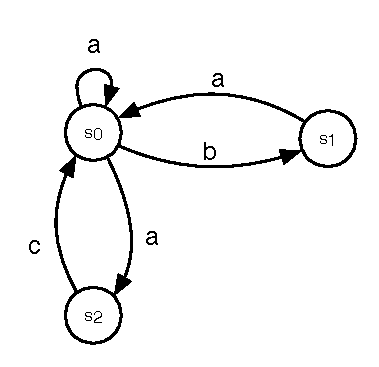
\includegraphics[scale=0.75]{Figs/examplesThesisLTS.pdf} 
   % \vspace{-1cm}
    \caption{Ejemplo de LTS.}
    %\vspace{-0.8cm}
    \label{figure:lts1}
\end{center}
\end{figure}
Con $|S|$ y $|{\rightarrow}|$ denotamos la cantidad de estados y arcos, respectivamente. Definimos $\post(s) = \{s' \in S \mid s \xrightarrow{e} s' \}$ como el conjunto de sucesores de $s$. Similarmente,  $\pre(s') = \{s \in S \mid s \xrightarrow{e} s' \}$ denota el conjunto de predecesores de $s'$.
Además, $\post^{*}(s)$ denota los estados alcanzables desde $s$.
Sin perder generalidad, requerimos que todo estado $s$ tenga un sucesor, i.e., $\forall s \in S : \post(s) \neq \emptyset$. Decimos que un LTS es \emph{determinista} si, para toda terna de estados  $s,t, t'$ y para toda etiqueta $e$, $s \xrightarrow{e} t$ y $s \xrightarrow{e} t'$ implica $t=t'$. 

Una \emph{ejecución} en un sistema de transición de estados $A$ es un camino infinito $\rho = \rho_0 \sigma_0 \rho_1 \sigma_1  \rho_2 \sigma_2 \dots \in (S \cdot \Sigma)^{w}$ 
donde $\rho_0 = \InitState$ y para todo $i$, $\rho_i \xrightarrow{\sigma_i} \rho_{i+1}$. De ahora en mas, dada una tupla $(x_0,\dots,x_n)$, denotaremos a $x_i$ con  $\pr{i}{x_0,\dots,x_n}$.



\section{Sistemas de Transición Probabilistas} 

Para definir estos sistemas primero es necesario definir distribuciones de probabilidad.

Una \emph{distribución de probabilidad} (discreta) $\mu$ sobre un conjunto numerable $S$ es una función $\mu: S \rightarrow [0, 1] $  tal que $\mu(S) \triangleq \sum_{s \in S} \mu(s) = 1$. 
Sea $\Dist(S)$ el conjunto de todas las distribuciones de probabilidad sobre $S$. $\Dirac_s \in \Dist(S)$ denota la distribución Dirac para $s$, i.e., $\Dirac_s(s) =1$ y $\Dirac_s(s') = 0$ siempre que $s'\neq s$.
El conjunto \textit{soporte} de $\mu$ se define como $\support{\mu} = \{s |~\mu (s) > 0\}$.


Un \emph{Sistema de Transición Probabilista} (PTS) es una estructura $A = \langle S, \Sigma, \rightarrow, s_0 \rangle$ 
donde 
\begin{enumerate}
\item%
  $S$ es el conjunto numerable de \emph{estados} que contiene el
  \emph{estado inicial} $s_0 \in S$,
\item%
  $\Sigma$ es un conjunto de \emph{acciones}, y
\item%
  ${\rightarrow} \subseteq S \times \Sigma \times \Dist(S)$ es una
  \emph{relación de transición (probabilista)}.
\end{enumerate}
Asumimos que desde cualquier estado siempre existe alguna transición saliente.

\begin{figure}[ht] 
\begin{center}
    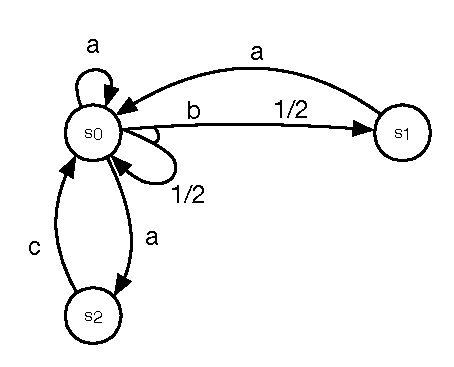
\includegraphics[scale=0.75]{Figs/examplesThesisPTS.pdf} 
   % \vspace{-1cm}
    \caption{Ejemplo de PTS.}
    %\vspace{-0.8cm}
    \label{figure:pts1}
\end{center}
\end{figure}
%In order to consider \textit{time}, we will distinguish the action $\text{tick} \in S$ which 
%represents a unit of time, and request that the PTS is deterministic on tick, that is, 
%for all $s \in S$ and $\mu, \mu' \in \Dist(S)$, if $s \xrightarrow{\text{tick}} \mu$ and 
%and $s \xrightarrow{\text{tick}} \mu'$, then $\mu = \mu'$.

Una distribución $w \in \Dist(S \times S')$ se dice que es un \textit{coupling} para $(\mu, \mu')$, con 
$\mu \in \Dist(S)$ y $\mu' \in \Dist(S')$, si $w(S, \cdot) = \mu'$ y 
$w(\cdot, S') = \mu$. $\couplings{\mu}{\mu'}$ denota el conjunto de todos los couplings para $(\mu, \mu')$.  Es de destacar que este conjunto define un politopo. $\vertices{\couplings{\mu}{\mu'}}$ denota el conjunto de todos los vértices del politopo correspondiente.
Este conjunto es finito si $S$ y $S'$ son finitos.
%
Para $R \subseteq S \times S'$, decimos que un coupling $w$ para $(\mu, \mu')$ 
\textit{respeta} $R$ si $\support{w} \subseteq R$ (i.e., $w(s, s') > 0 \Rightarrow s~R~s'$).
Definimos $\RelCoupling \subseteq \Dist(S) \times \Dist(S')$ por $\mu~\RelCoupling~\mu'$ si y solo si
existe un coupling $R$-respetuoso para $(\mu, \mu')$.%, for all $\mu \in \Dist(S)$ and $\mu' \in \Dist(S')$. 

\section{Conceptos Básicos de Teoría de la Medida}

En esta sección se introducen conceptos básicos de Teoría de la Medida que son necesarios para el resto de la tesis.

Un \emph{$\sigma$-álgebra} sobre un conjunto $\Omega$ es un conjunto $\mathcal{F} \subseteq \mathcal{P}(\Omega)$ tal que:
\begin{enumerate}
\item $\Omega \in \mathcal{F}$
\item $A \in \mathcal{F} \implies A^\mathsf{c} \in \mathcal{F}$
\item $A_n \in \mathcal{F}$, para todo $n \geq 0$, $ \implies \bigcup_{n \geq 0}A_n \in \mathcal{F}$
\end{enumerate}
El par $(\Omega,\mathcal{F})$ se denomina \emph{espacio medible}.
Las $\sigma$-álgebras sirven como dominio sobre las probabilidades. En tal caso $\Omega$ corresponde al espacio muestral, y los elementos de $\mathcal{F}$ corresponden a los eventos cuya probabilidad queremos medir. Un ejemplo de espacio medible seria un dado, donde $\Omega=\{1,2,3,4,5,6\}$ y $\mathcal{F}=\mathcal{P}(\Omega)$.

Sea $\mathcal{A} \subseteq \mathcal{P}(\Omega)$. La \emph{$\sigma$-álgebra generada por $\mathcal{A}$} se define como $\sigma(\mathcal{A}) = \bigcap\{\mathcal{F} \subseteq \mathcal{P}(\Omega) \mid \mathcal{F}$ es una $\sigma$-álgebra y $\mathcal{A} \subseteq \mathcal{F}\}$. Volviendo al ejemplo del dado, su $\sigma$-álgebra puede ser generada por el conjunto $\{\{1\},\{2\},\{3\},\{4\},\{5\},\{6\}\}$. La $\sigma$-álgebra sobre los reales que usamos cotidianamente en probabilidades es generada por el conjunto $\mathcal{C} = \{(a,b] \mid a,b \in \mathbb{R} \cup \{-\infty,\infty\}\}$. A $\sigma(\mathcal{C})$ se la denomina \textit{$\sigma$-álgebra de Borel} sobre los reales.

Sea $\mathcal{A} \subseteq \mathcal{P}(\Omega)$ con $\emptyset \in \mathcal{A}$. Se denomina \emph{medida} a una función $\mu:\mathcal{A} \rightarrow [0,\infty]$ tal que:
\begin{enumerate}
\item $\mu(\emptyset) = 0$
\item si $\{A_n\}_{n \in \mathbb{N}} \subseteq \mathcal{A}$ es una familia de conjuntos disjuntos de a pares, y además $\biguplus_{n \in \mathbb{N}} A_n \in \mathcal{A}$, luego $\mu(\biguplus_{n \in \mathbb{N}} A_n) = \Sigma_{n \in \mathbb{N}} \mu(A_n)$.
\end{enumerate}
Si además, $\mu(\Omega) = 1$, $\mu$ es una medida de probabilidad.

Sean $(\Omega_1,\mathcal{F}_1)$ y $(\Omega_2,\mathcal{F}_2)$ dos espacios medibles, una función $f:\Omega_1 \rightarrow \Omega_2$ se dice que es \emph{medible} si $\forall B \in \mathcal{F}_2 : f^{-1}(B) \in \mathcal{F}_1$.

\section{Juegos}

Vamos a introducir algunas definiciones y resultados básicos sobre teoría de juegos que serán necesarios para el capítulo~\ref{cap:maskingMeasure}, el lector interesado puede ver \cite{AptG11}.

Un \emph{grafo de juego} $G$ es una tupla $G = \langle V, V_1, V_2, E, \InitVertex \rangle$ donde $V$ es un conjunto de vértices, $E\subseteq V \times V$ es un conjunto de arcos, $\InitVertex$ es el vértice inicial del juego, y $(V_1, V_2)$ es una partición de $V$. Intuitivamente, el grafo representa un juego entre dos jugadores, donde un token se coloca inicialmente en el vértice inicial, y luego sigue por rondas. Si el token esta en un vértice $v \in V_1$, entonces el jugador $1$ elige un arco $(v, w) \in E$ y mueve el token al vértice $w$. En caso de que el token este en un vértice $v \in V_2$, entonces la elección es del jugador $2$.

Un \emph{grafo de juego con costos} es un grafo de juego mas una función de costo (o recompensa) $\reward^G:V \rightarrow \mathbb{R}$. Un camino maximal en el grafo de juego $G$ se denomina una \emph{jugada}. El conjunto de todas las jugadas se denota con $\Omega$. Los \emph{grafos de juego deterministas} se definen de la misma manera que en sistemas de transición de estados. Además, utilizaremos la notación $\post(v)$ para denotar los sucesores del vértice $v$, y $\pre(v)$ para denotar a los predecesores del vértice $v$.

Dado un grafo de juego $G$, una \emph{estrategia} para el jugador $1$ es una función $\pi: V^{*} V_1 \rightarrow V$ tal que para todo  $\rho_0  \rho_1 \dots \rho_i \in V^{*} V_1$, tenemos que si $\pi(\rho_0  \rho_1\dots \rho_i) = \rho $, entonces $(\rho_i, \rho) \in E$. Una estrategia para el jugador $2$ se define similarmente. El conjunto de todas las estrategias para el jugador $p$ (para $p \in \{1,2\}$) se denota por $\Pi_{p}$.
Una estrategia para el jugador $p$ se dice \emph{sin memoria} (o posicional, o estacionaria) si puede ser definida por un mapping $f:V_p \rightarrow V$, de tal forma que si $v \in V_p$ entonces $(v, f(v)) \in E$.
Lo cual significa que estas estrategias no necesitan memoria del historial de movimientos previos al estado corriente. Además, una jugada $\rho_0 \rho_1 \rho_2 \dots$ se dice que se conforma a una estrategia $\pi$ del jugador $p$ si $\forall i \geq 0: (\rho_i \in V_p) \Rightarrow  \pi(\rho_0 \rho_1 \dots \rho_i) = \rho_{i+1}$. El \emph{resultado} de una estrategia $\pi_{1}$ del jugador $1$ y una estrategia $\pi_{2}$ del jugador $2$ es la jugada única, denominada $\out(\pi_1, \pi_2)$, que se conforma tanto a $\pi_1$ como a $\pi_2$.

Un \emph{juego} se compone de un grafo de juego y un objetivo Booleano (o cualitativo) o un objetivo cuantitativo. Un \emph{objetivo booleano} es una función $\Phi: \Omega \rightarrow \{0, 1\}$ y la meta del jugador $1$ en un juego con un objetivo $\Phi$ es seleccionar una estrategia de tal forma que el resultado del juego sea $1$, independientemente de lo que haga el jugador $2$. Por el contrario, la meta del jugador $2$ es asegurarse que el resultado sea $0$. Dado un objetivo booleano $\Phi$, una jugada $\rho$ es \emph{ganadora} para el jugador $1$ (resp. jugador $2$) si  $\Phi(\rho) = 1$ (resp. $\Phi(\rho) = 0$). Una estrategia $\pi$ es una \emph{estrategia ganadora} para el jugador $p$ si toda jugada que se conforme a $\pi$ es ganadora para el jugador $p$. Decimos que un juego con objetivo booleano esta \emph{determinado} si algún jugador tiene una estrategia ganadora, y decimos que está \emph{determinado sin memoria} si esa estrategia ganadora es estacionaria. Los juegos de alcanzabilidad son aquellos juegos cuyos objetivos están definidos como $\Phi(\rho_0 \rho_1 \rho_2 \dots) = (\exists i : \rho_i \in B)$ para algún conjunto $B \subseteq V$, un resultado estándar de los juegos de alcanzabilidad es que son determinados sin memoria.

Un \emph{objetivo cuantitativo} esta dado por una función de \emph{payoff} $f: \Omega \rightarrow \mathbb{R}$ y la meta del jugador $1$ es maximizar el valor $f$ de la jugada, mientras que la meta del jugador $2$ es minimizar este valor. Para un objetivo cuantitativo $f$, el valor del juego para la estrategia $\pi_1$ del jugador $1$, denotado por $v_1(\pi_1)$, se define como el ínfimo sobre todos los valores resultantes de estrategias del jugador $2$, i.e., $v_1(\pi_1) = \inf_{\pi_2 \in \Pi_2} f(\out(\pi_1, \pi_2))$. El valor del juego para el jugador $1$ se define como el supremo de los valores de todas las estrategias del jugador $1$, i.e., $\sup_{\pi_1 \in \Pi_1} v_1(\pi_1)$. Análogamente, el valor del juego para una estrategia $\pi_2$ del jugador $2$ y el valor del juego para el jugador $2$ se definen como $v_2(\pi_2) = \Sup_{\pi_1 \in \Pi_1} f(\out(\pi_1, \pi_2))$ 
y $\inf_{\pi_2 \in \Pi_2} v_2(\pi_2)$, respectivamente.
Una estrategia es \emph{optimal} para un jugador si el valor de la estrategia para ese jugador es igual al valor del juego para ese jugador. Decimos que un juego esta determinado si los valores del juego para ambos jugadores es igual, es decir:
$\sup_{\pi_1 \in \Pi_1} v_1(\pi_1) = \inf_{\pi_2 \in \Pi_2} v_2(\pi_2)$. En este caso denotamos con $\val(\mathcal{G})$ al valor del juego $\mathcal{G}$.
Existe un resultado importante \cite{Martin98} que caracteriza un conjunto grande de juegos determinados y establece que cualquier juego con una función cuantitativa $f$ que esté acotada y sea Borel-medible esta determinado.
Cuando el grafo de juego es visible en su totalidad por ambos jugadores, se dice que el juego es de información perfecta. Cuando el grafo de juego está particionado en vértices de distintos jugadores, se dice que el juego es por turnos.
Por último, se dice que el juego es de suma-cero cuando en cada jugada lo que gana un jugador, el otro lo pierde en igual cantidad. Los juegos que definimos en esta tesis son de información perfecta, por turnos y suma-cero.

\section{Juegos Estocásticos}

En esta sección introducimos algunas definiciones básicas y resultados sobre juegos estocásticos que serán necesarias para el capítulo \ref{cap:fairAdversaries}.

Una \emph{distribución de probabilidad} (discreta) $\mu$ sobre un conjunto numerable $S$ es una función $\mu: S \rightarrow [0, 1] $  tal que 
$\mu(S) = \sum_{s \in S} \mu(s) = 1$. 
Vamos a denotar como $\Dist(S)$ al conjunto de todas las distribuciones de probabilidad sobre $S$. $\Delta_s \in \Dist(S)$ denota la distribución Dirac para $s$, i.e., 
$\Delta_s(s) =1$ y $\Delta_s(s') = 0$ para $s'\neq s$.
El conjunto \textit{soporte} de $\mu$ se define como $\support{\mu} = \{s |~\mu (s) > 0\}$.

Dado un conjunto $V$, $V^*$ (resp. $V^\infty$) denota el conjunto de todas las secuencias finitas (resp. secuencias infinitas ) de elementos de $V$. La concatenación será representada usando yuxtaposición. Usamos las variables $\omega, \omega', \dots \in V^\infty$ para hacer referencia a secuencias infinitas, y las variables $\hat{\omega}, \hat{\omega}', \dots \in V^*$ para hacer referencia a secuencias finitas. El $i$-ésimo elemento de una secuencia finita (resp. infinita) $\hat{\omega}$ (resp. $\omega$) se denota como
$\hat{\omega}_i$ (resp. $\omega_i$). Además, para cualquier secuencia finita $\hat{\omega}$, $|\hat{\omega}|$ denota su longitud. Para $\omega \in V^\infty$, $\inf(\omega)$ denota el conjunto de ítems que aparecen con infinita frecuencia en $\omega$. Dado
$S \subseteq V^*$, $S^k$ es el conjunto obtenido al concatenar las secuencias de $S$ $k$ veces.
	 
Un \emph{juego estocástico} \cite{ChatterjeeH12,SvorenovaKwiatkowska16} es una tupla $\StochG = ( V,  (V_1, V_2, V_\Probabilistic), \delta  ) $, donde $V$ es un conjunto finito de vértices (o estados) con $V_1, V_2, V_\Probabilistic \subseteq V$ siendo una partición de $V$, y $\delta : V \times V \rightarrow [0,1]$ es una función de transición probabilista, tal que para todo $v \in V_1\cup V_2$, $\delta(v,v') \in  \{0,1\}$, para todo $v' \in V$; y $\delta(v,\cdot) \in \Dist(V)$ para todo $v \in V_\Probabilistic$.
Si $V_\Probabilistic = \emptyset$, entonces $\mathcal{G}$ se denomina \emph{grafo de juego de $2$ jugadores}. Además, si $V_1 = \emptyset$ o $V_2 = \emptyset$, entonces $\mathcal{G}$ es un \emph{proceso de decisión de Markov} (o MDP). Finalmente, en el caso de que $V_1= \emptyset$ y $V_2 = \emptyset$, $\mathcal{G}$ es una \emph{cadena de Markov} (o MC). Para todos los estados $v \in V$ definimos $\post^\delta(v) = \{v' \in V \mid \delta(v,v')>0 \}$, como el conjunto de sucesores de $v$. De forma similar, $\pre^\delta(v') = \{v \in V \mid \delta(v,v')>0 \}$ denota el conjunto de predecesores de $v'$, omitimos el índice $\delta$ cuando está claro por el contexto. También, cuando sea útil, fijaremos un estado inicial para el juego, en tal caso usaremos la notación $\mathcal{G}_v$ para indicar que el juego empieza en $v$. Además, asumimos que $\post(v) \neq \emptyset$ para todo
$v \in V$.
Un vértice $v \in V$ se denomina \emph{terminal} si $\delta(v,v) = 1$, y $\delta(v,v')=0$ para todo $v \neq v'$.
La mayoría de resultados sobre MDPs se basan en la noción de \emph{componente final} \cite{BaierK08}, extendemos esta noción de manera directa para juegos estocásticos de 2 jugadores: una componente final de $\StochG$ es un par $(V',\delta')$ tal que (a) $V' \subseteq V$; (b) $\delta'(v) = \delta(v)$ para $v \in V_\Probabilistic$; (c) $\emptyset \neq \post^{\delta'}(v) \subseteq \post^\delta(v)$ para $v \in V_1 \cup V_2$; (d) $\post^{\delta'}(v) \subseteq V'$ para todo $v \in V'$; (e) el grafo subyacente a $(V',\delta')$ es fuertemente conexo.  Notemos que una componente final también puede ser considerada como un juego. El conjunto de componentes finales de $\StochG$ se denota como $\EndComp(\StochG)$.
 
%
%	 Another way of defining stochastic games is by partitioning the state space into Player 1 and Player 2 states and	considering a set of possible actions for the players. In this setting, the transition function assigns a probability distribution for each pair $(s,a)$ composed of a state and an action. Note that this definition (used, for instance, in \cite{FilarV96})  is equivalent to the definition given above \cite{SvorenovaKwiatkowska16}.
%From now on, given a tuple $(x_0,\dots,x_n)$, we denote $x_i$ by $\pr{i}{x_0,\dots,x_n}$. 
%
Un \emph{camino} en el juego estocástico $\StochG$ es una secuencia infinita de vértices $v_0 v_1 \dots$ tal que $\delta(v_k, v_{k+1})>0$ para todo $k \in \mathbb{N}$.
 %% The set of all paths is named $\GamePaths_{\StochG}$, and the set of finite prefixes of paths is denoted $\FinGamePaths_{\StochG}$. Similarly, the set of  paths starting at vertex $v$ is written $\GamePaths_{\StochG,v}$, and $\FinGamePaths_{\StochG,v}$ denotes the set of finite paths starting at $v$.
$\GamePaths_{\StochG}$ denota al conjunto de todos los caminos, y $\FinGamePaths_{\StochG}$ denota el conjunto de prefijos finitos de caminos. 
Similarmente, $\GamePaths_{\StochG,v}$  y  $\FinGamePaths_{\StochG,v}$ denota al conjunto de caminos y el conjunto de caminos finitos que comienzan en $v$.
	 
%The set of all plays is denoted by $\Omega$,
%and the set of plays starting in a vertex $v$ is written $\Omega_v$. The set of states appearing an infinite number of times in %a play $\omega$ is denoted $\inf(\omega)$.

Una \emph{estrategia} para el Jugador $i$ (para $i\in\{1,2\}$) en un juego $\StochG$ es una función $\strat{i}: V^*  V_i \rightarrow \Dist(V)$ que asigna una distribución probabilista a cada secuencia finita de estados tal que $\strat{i}(\hat{\omega}v)(v') > 0$ solo si $v' \in \post(v)$. El conjunto de todas las estrategias para el Jugador $i$ se denota $\Strategies{i}$. Una estrategia $\strat{i}$ se denomina \emph{pura} o \emph{determinista} si, para cada $\hat{\omega} v \in V^*V_i$, $\strat{i}(\hat{\omega} v)$  es una distribución Dirac, y se le llama \emph{sin memoria} si $\strat{i}(\hat{\omega} v) = \strat{i}(v)$, para todo $\hat{\omega} \in V^*$.
%
%% The set of all the memoryless strategies for Player $i$ is denoted $\MemorylessStrats{i}$,
%% $\DetStrats{i}$ denotes the set of deterministic strategies, and $\DetMemorylessStrats{i}$ denotes the set of all deterministic and memoryless strategies for that player.
%
Sean $\MemorylessStrats{i}$ y $\DetStrats{i}$ el conjunto de todas las estrategias sin memoria y el conjunto de todas las estrategias deterministas respectivamente para el Jugador $i$.  $\DetMemorylessStrats{i} = \MemorylessStrats{i} \cap \DetStrats{i}$ es el conjunto de todas sus estrategias deterministas y sin memoria.

Dadas dos estrategias $\strat{1} \in \Strategies{1}$, $\strat{2} \in \Strategies{2}$ y un vértice inicial $v$,  el \emph{resultado} del juego es una cadena de Markov \cite{ChatterjeeH12}, denotada 
$\StochG^{\strat{1}, \strat{2}}_v$. Un evento $\mathcal{A}$ es un conjunto medible en la $\sigma$-álgebra de Borel generada por los conos de $\GamePaths_{\StochG}$. El \emph{cono} o \emph{cilindro} derivado del camino finito $\hat{\omega} \in \FinGamePaths_{\StochG}$ es el conjunto $\cone(\hat{\omega})=\{\omega \in \GamePaths_\StochG \mid \forall 0 \leq i < |\hat{\omega}|: \omega_i = \hat{\omega}_i \}$. $\Prob{\strat{1}}{\strat{2}}_{\StochG,v}$ es la medida de probabilidad asociada que se obtiene al fijar las estrategias $\strat{1}$, $\strat{2}$, y un vértice inicial $v$  \cite{ChatterjeeH12}. Intuitivamente, $\Prob{\strat{1}}{\strat{2}}_{\StochG,v}(\mathcal{A})$
es la probabilidad de que las estrategias $\strat{1}$ y $\strat{2}$ generen un camino que pertenezca al conjunto $\mathcal{A}$ cuando el juego $\StochG$ comienza en $v$. Cuando no haya lugar a dudas, denotaremos simplemente $\Prob{\strat{1}}{\strat{2}}_{\StochG,v}(\hat{\omega})$ en lugar de $\Prob{\strat{1}}{\strat{2}}_{\StochG,v}(\cone(\hat{\omega}))$.
%Similarly, $\Paths{\strat{1}}{\strat{2}}_{\StochG, v}$ is the set of paths
%of $\StochG^{\strat{1}, \strat{2}}$ starting at vertex $v$ (i.e., the plays generated by strategies $\strat{1}$ and $\strat{2}%$). Similarly,  $\FinPaths{\strat{1}}{\strat{2}}_{\StochG, v}$ denotes the set of finite paths generated by the strategies. Also, 
Para MDPs y MCs usaremos notaciones similares. Un juego estocástico (como se ha definido anteriormente) se dice que es \emph{terminante} \cite{Condon92} si para todo par de estrategias $\strat{1}, \strat{2}$ la probabilidad de alcanzar un estado terminal es $1$. Usamos notación {\LTL} para representar conjuntos específicos de caminos, por ejemplo, $\Diamond T = \{\omega \in \GamePaths_{\StochG} \mid \exists i \geq 0 : \omega_i \in T \}$ es el conjunto de todas las jugadas del juego que alcanzan vértices en $T$.

%  Given a game, a vertex $v \in V$ is said to be \emph{terminal} if $\delta(v,v) = 1$, and $\delta(v,v')=0$ for all $v \neq v'$. A stochastic game (defined as above) is said to be \emph{stopping} \cite{Condon92} if 
%for all pair of strategies $\strat{1}, \strat{2}$ the probability of reaching a terminal state is $1$.


%[RD2ALL] Review this last paragraph, may more explanation is needed, page 398 paper ChatterjeeH12

%A \emph{Boolean objective} for $\mathcal{G}$ is a set $\Phi \subseteq \Omega$, we say that a play $\omega$ is winning for Player $1$ at vertex $v$ if $\omega \in \Phi$, otherwise it is winning for Player $2$ 
%(i.e., we only consider \emph{zero-sum} games).   A strategy $\strat{1}$ is a \emph{sure winning strategy} for Player $1$  from vertex $v$ if, for every strategy $\strat{2}$ for Player $2$, $\out_v(\strat{1}, \strat{2}) \subseteq \Phi$. $\strat{1}$ is said to be \emph{almost-sure winning} if for every strategy $\strat{2}$ for Player $2$, we have $\Prob{\strat{1}}{\strat{2}}(\Phi)=1$.
%	Sure  and almost-sure winning strategies for Player $2$ are defined in a similar way.
%Reachability games are games with Boolean objectives of the style: 
%$\Phi = \{ \omega_0,\omega_1,\dots \in \Omega \mid  \exists i : \omega_i \in V' \}$, for some set $V' \subseteq V$. A standard result is that, if a reachability game has a sure winning strategy, then
%it has a pure memoryless sure winning strategy \cite{ChatterjeeH12}. 

Para juegos estocásticos definimos el \emph{objetivo cuantitativo} de manera análoga a los juegos no estocásticos, es decir, como una función medible $f: V^{\infty} \to \mathbb{R}$.   Sea $\Expect{\strat{1}}{\strat{2}}_{\StochG,v}[f]$ el valor esperado de la función medible $f$ bajo la probabilidad $\Prob{\strat{1}}{\strat{2}}_{\StochG,v}$, el objetivo del Jugador $1$ es maximizar este valor mientras que la meta del Jugador $2$ es minimizarlo.  A veces las funciones de objetivo cuantitativo pueden ser definidas a través de \emph{recompensas}. Estas son asignadas por una \emph{función de recompensa} $\reward:V \to \mathbb{R}^+$. Un \emph{juego estocástico con recompensas} es una tupla $(V, (V_1, V_2, V_\Probabilistic), \delta, \reward \rangle$ compuesta de un juego estocástico y una función de recompensa. Asumimos que para todo vértice terminal $v$,  $\reward(v) = 0$.
%Unless stated otherwise, we assume that  $\reward(v) = 0 $ for all terminal vertices $v$.

El valor del juego para el Jugador $1$ en el vértice $v$ bajo la estrategia $\strat{1}$ se define como el ínfimo sobre todos los valores que resultan de estrategias del Jugador $2$ en ese vértice, i.e. $\inf_{\strat{2} \in \Strategies{2}} \Expect{\strat{1}}{\strat{2}}_{\StochG,v}[f]$.
El \emph{valor del juego} para el Jugador $1$ se define como el supremo de todos los valores que resultan de estrategias del Jugador $1$, i.e., $\sup_{\strat{1} \in \Strategies{1}} \inf_{\strat{2} \in \Strategies{2}} \Expect{\strat{1}}{\strat{2}}_{\StochG,v}[f]$.
Análogamente, el valor del juego para el Jugador $2$ en el vértice $v$ bajo la estrategia $\strat{2}$ y el valor del juego para el Jugador $2$ se definen como $\sup_{\strat{1} \in \Strategies{1}}  \Expect{\strat{1}}{\strat{2}}_{\StochG,v}[f]$ 
y $\inf_{\strat{2} \in \Strategies{2}} \sup_{\strat{1} \in \Strategies{1}}  \Expect{\strat{1}}{\strat{2}}_{\StochG,v}[f]$, respectivamente. Decimos que un juego está \emph{determinado} si ambos valores son iguales, es decir,
	$\sup_{\strat{1} \in \Strategies{1}} \inf_{\strat{2} \in \Strategies{2}} \Expect{\strat{1}}{\strat{2}}_{\StochG,v}[f]
	=
	\inf_{\strat{2} \in \Strategies{2}} \sup_{\strat{1} \in \Strategies{1}} \Expect{\strat{1}}{\strat{2}}_{\StochG,v}[f]$.
%% \[
%% 	\sup_{\strat{1} \in \Strategies{1}} \inf_{\strat{2} \in \Strategies{2}} \Expect{\strat{1}}{\strat{2}}_{\StochG,v}[f]
%% 	=
%% 	\inf_{\strat{2} \in \Strategies{2}} \sup_{\strat{1} \in \Strategies{1}} \Expect{\strat{1}}{\strat{2}}_{\StochG,v}[f].
%% \]
Martin \cite{Martin98} demostró la determinación de juegos estocásticos para funciones de objetivo acotadas y Borel-medibles.
%ESTO DE ABAJO HABLA DEL CAP 5
En esta tesis nos enfocamos en la función de payoff de \emph{recompensa total acumulada}, i.e.: $\Rewards(\omega) = \sum^\infty_{i=0} \reward(\omega_i)$. Debido a que $\Rewards$ no esta acotada, los resultados de Martin \cite{Martin98} no aplican a esta función. Nos restringimos a recompensas no negativas, como se verá mas adelante, las recompensas no negativas bastan para lidiar con casos de estudio interesantes, discutiremos brevemente en las conclusiones una posible extensión de los resultados presentados aquí a juegos con recompensas negativas.
%	The following result from \cite{Martin98} characterizes a large set of determined games.
%\begin{theorem} Any stochastic game with a quantitative function $f$ that is bounded and Borel measurable is determined. That is:
%\[
%	\sup_{\sigma \in \Sigma} \inf_{\pi \in \Pi}  \Expect{\sigma}{\pi} [f]   =  \inf_{\pi \in \Pi} \sup_{\sigma \in \Sigma} \Expect{\sigma}{\pi}[f]
%\]
%\end{theorem}



	

